\makeatletter
\makeatother
\documentclass[../main.tex]{subfiles}

\graphicspath{
    {img}
	{../img/}
}

\begin{document}
\section{Метод Римана для решения обобщённой задачи Коши для гиперболического уравнения}

Мы праябаліся і прапусцілі яго :( Таму замест тэха Рымана тут скрыншоты канспекту Лізы

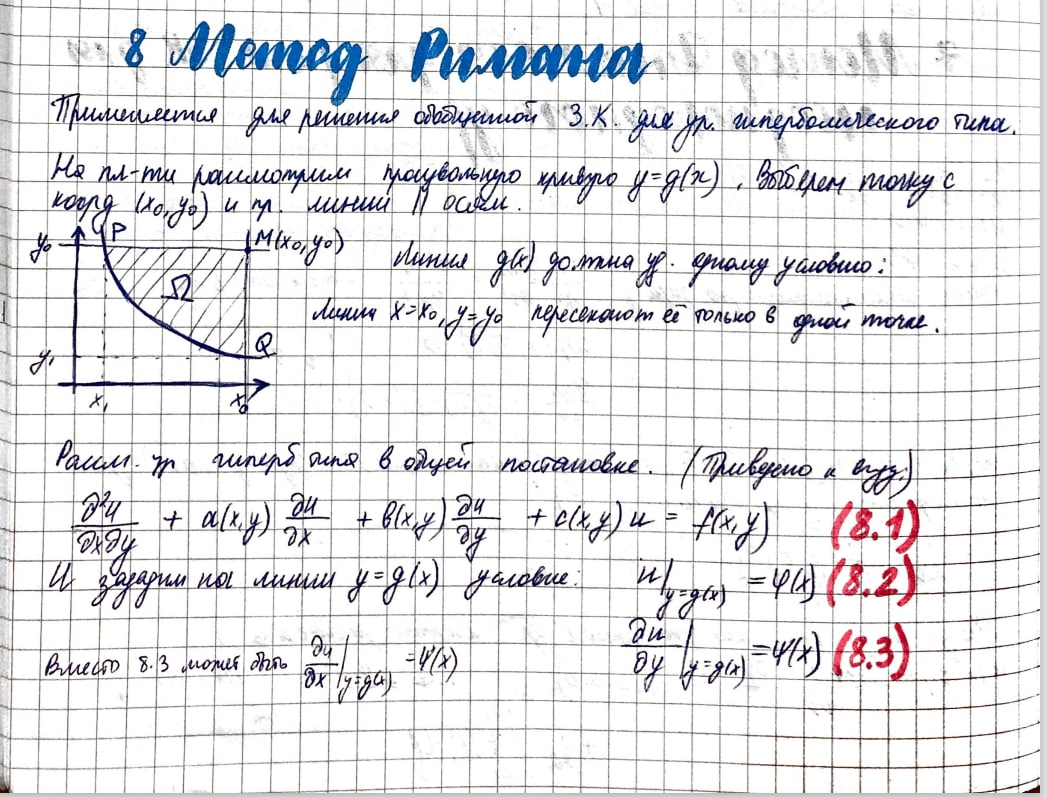
\includegraphics[scale=0.7]{Liza_2.7.1.jpg}
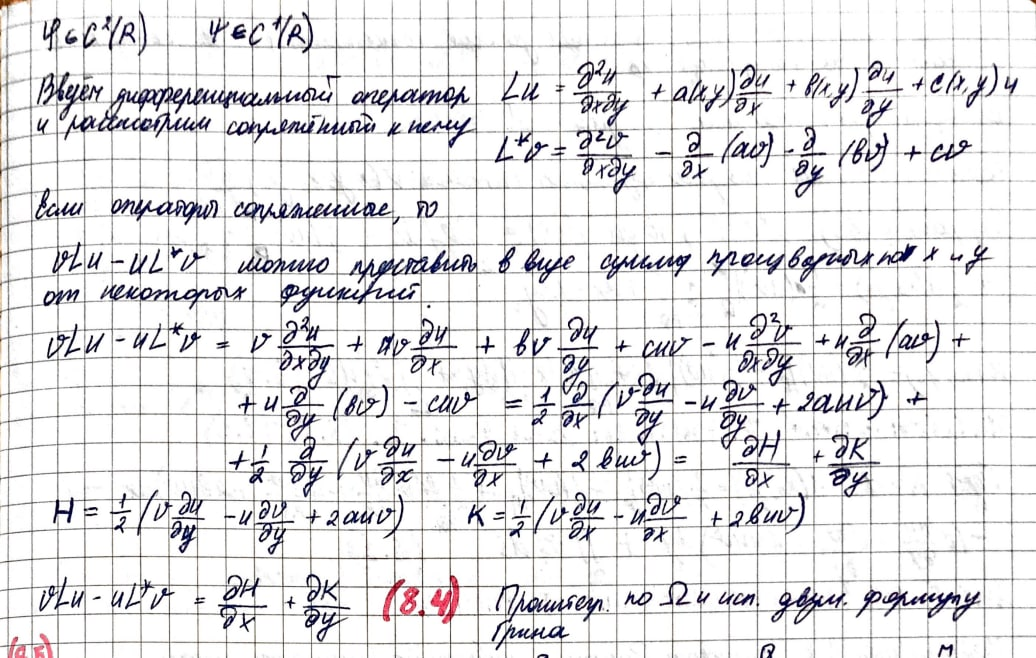
\includegraphics[scale=0.7]{Liza_2.7.2.jpg}
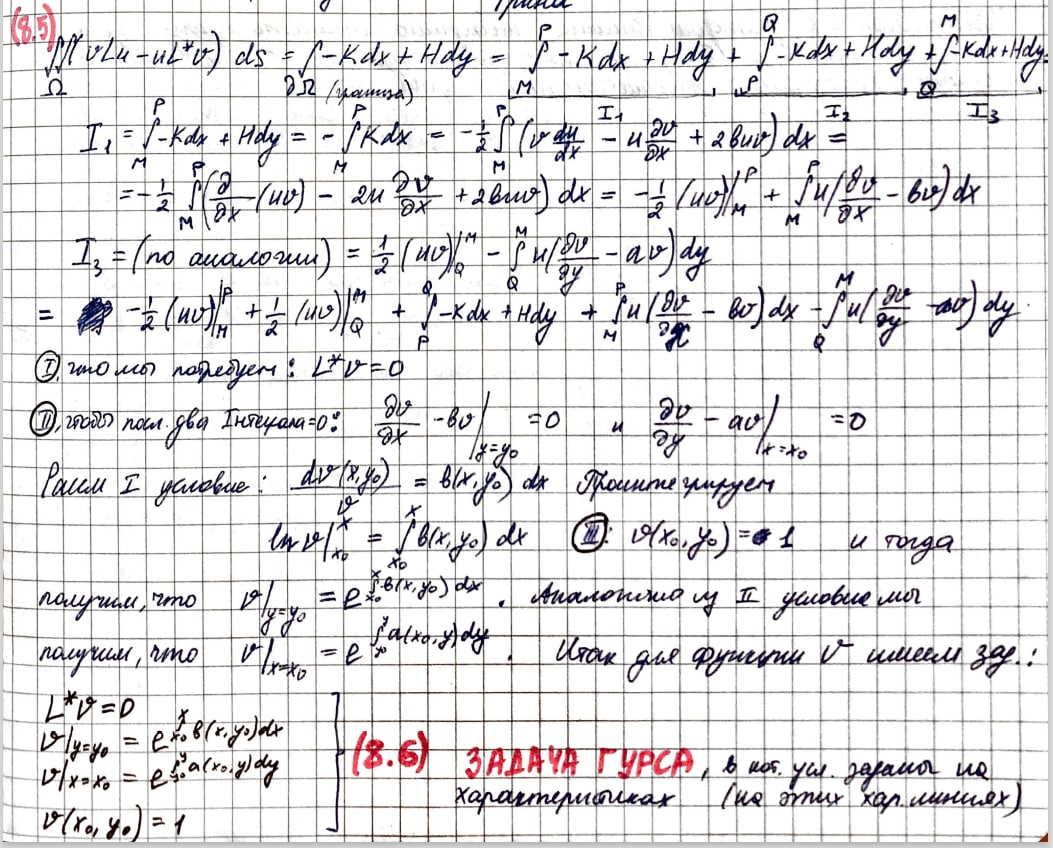
\includegraphics[scale=0.7]{Liza_2.7.3.jpg}
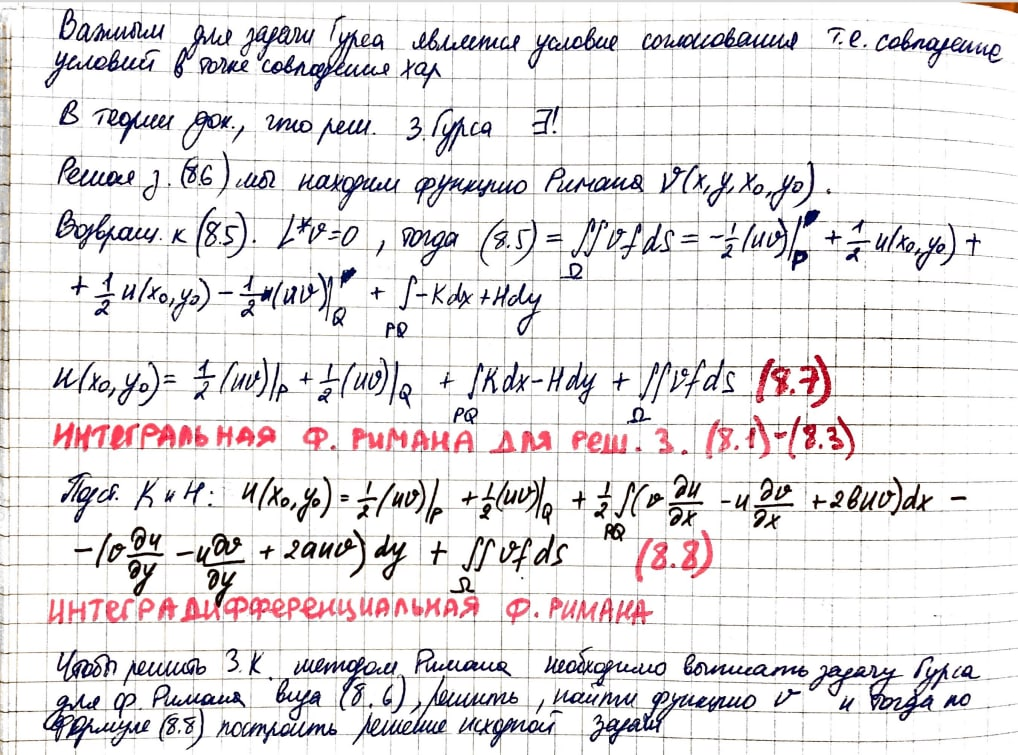
\includegraphics[scale=0.7]{Liza_2.7.4.jpg}
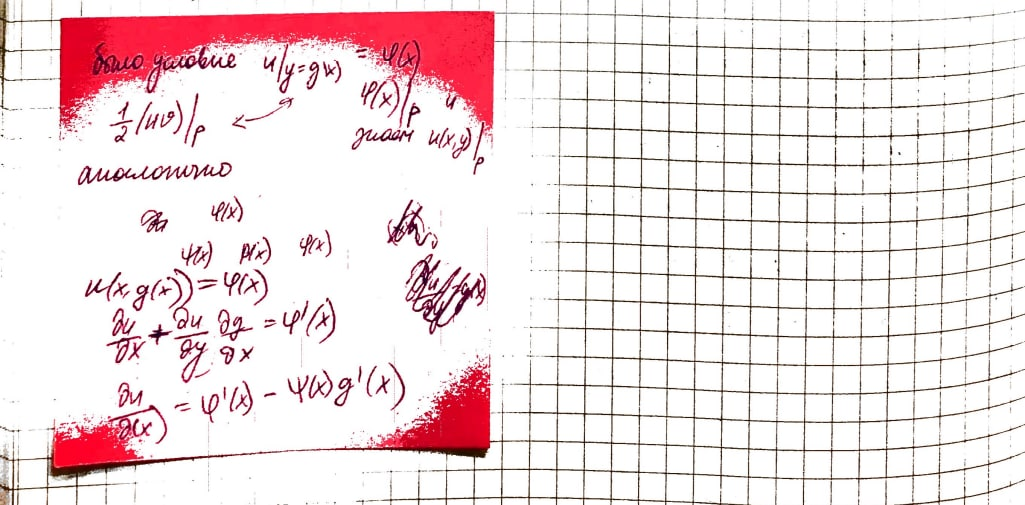
\includegraphics[scale=0.7]{Liza_2.7.5.jpg}

WIP
Рассмотрим уравнение гиперболического типа в общей постановке:
\begin{gather}
    \label{eq:2.7.1}
    \pderivtwo{u}{x}{y} + a\pderiv{u}{x} +b\pderiv{u}{y} + cu = f(x,y)\\
    \label{eq:2.7.2}
    u|_{y=g(x)} = \varphi(x)\\
    \pderiv{u}{y}|_{y=g(x)} = \psi(x)
\end{gather}
Причём $y=g(x)$ пересекает прямые $x=x_0$, $y=y_0$ только в одной точке.

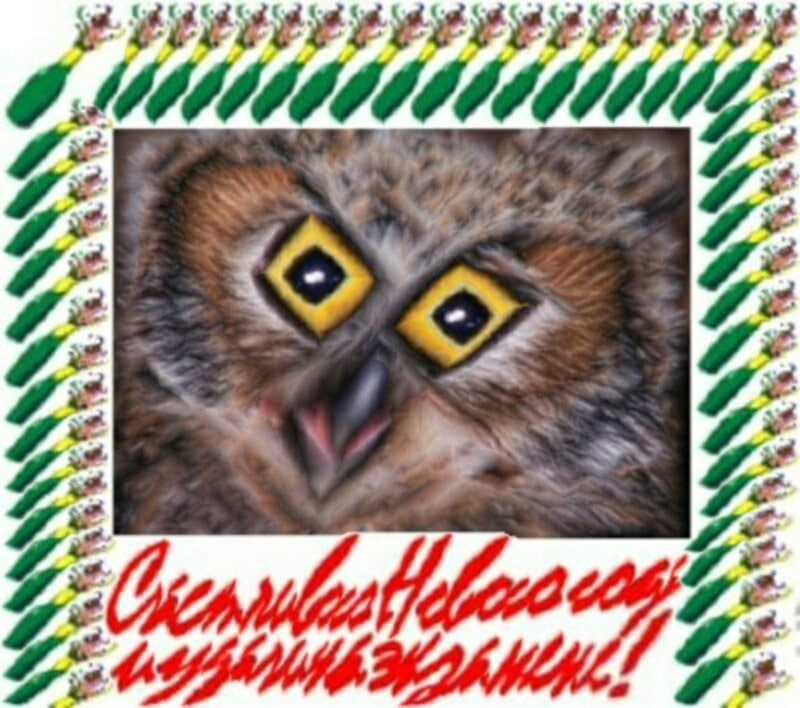
\includegraphics[scale=0.4]{example.jpg}



\end{document}